\section{Experimental Results}

\subsection*{Evaluation Metrics}
We use two metrics to measure model accuracy, using the cardiologist committee
annotations as the ground truth.

\textbf{Sequence Level Accuracy (F1):} We measure the average overlap between
the prediction and the ground truth sequence labels. For every record, a model
is required to make a prediction approximately once per second (every 256
samples). These predictions are compared against the ground truth annotation.

\textbf{Set Level Accuracy (F1):} Instead of treating the labels for a record
as a sequence, we consider the set of unique arrhythmias present in each 30
second record as the ground truth annotation. Set Level Accuracy, unlike
Sequence Level Accuracy, does not penalize for time-misalignment within a
record. We report the F1 score between the unique class labels from the ground
truth and those from the model prediction.

In both the Sequence and the Set case, we compute the F1 score for each class
separately. We then compute the overall F1 (and precision and recall) as the
class-frequency weighted mean.

\subsection*{Model and Cardiologist Performance}

We assess the cardiologist performance on the test set. Recall that each of the
records in the test set has a ground truth label from a committee of three
cardiologists as well as individual labels from a disjoint set of 6 other
cardiologists. To assess cardiologist performance for each class, we take the
average of all the individual cardiologist F1 scores using the group label as
the ground truth annotation.

\begin{table}
\centering
\begin{tabular}{r l l}
\toprule
                               & Sequence AUC (95\% CI)   & Set AUC (95\% CI) \\
\midrule
Atrial Fibrillation \& Flutter & 0.975 (0.968-0.982) & 0.959 (0.924-0.994) \\
Atrio-ventricular Block        & 0.989 (0.984-0.994) & 0.981 (0.954-1.000) \\
Bigeminy                       & 0.998 (0.995-1.000) & 0.997 (0.981-1.000) \\
Ectopic Atrial Rhythm          & 0.908 (0.883-0.932) & 0.935 (0.863-1.000) \\
Idioventricular Rhythm         & 0.995 (0.987-1.000) & 0.986 (0.958-1.000) \\
Junctional Rhythm              & 0.985 (0.978-0.992) & 0.980 (0.949-1.000) \\
Noise                          & 0.985 (0.979-0.992) & 0.958 (0.914-1.000) \\
Sinus Rhythm                   & 0.976 (0.973-0.980) & 0.981 (0.968-0.994) \\
Supraventricular Tachycardia   & 0.972 (0.959-0.985) & 0.940 (0.884-0.996) \\
Trigeminy                      & 0.999 (0.995-1.000) & 0.997 (0.979-1.000) \\
Ventricular Tachycardia        & 0.995 (0.981-1.000) & 0.981 (0.935-1.000) \\
Wenckebach                     & 0.982 (0.972-0.991) & 0.981 (0.948-1.000) \\
\midrule
   Average                     & 0.979               & 0.974 \\
\bottomrule
\end{tabular}
\caption{The model AUC scores with 95\% confidence intervals for the sequence
         and set level metrics.}
\label{tab:arrhythmias:model_auc}
\end{table}

\begin{table}
\centering
\begin{tabular}{r l l}
\toprule
             & Sensitivity       & Specificity  \\
             & (Specificity=0.9) & (Sensitivity=0.9) \\
\midrule
Atrial Fibrillation \& Flutter & 0.923 & 0.914 \\
Atrio-ventricular Block        & 0.991 & 0.964 \\
Bigeminy                       & 1.000 & 0.997 \\
Ectopic Atrial Rhythm          & 0.754 & 0.665 \\
Idioventricular Rhythm         & 0.990 & 0.990 \\
Junctional Rhythm              & 0.982 & 0.959 \\
Noise                          & 0.965 & 0.968 \\
Sinus Rhythm                   & 0.934 & 0.946 \\
Supraventricular Tachycardia   & 0.958 & 0.925 \\
Trigeminy                      & 1.000 & 0.999 \\
Ventricular Tachycardia        & 1.000 & 0.981 \\
Wenckebach                     & 0.977 & 0.956 \\
\bottomrule
\end{tabular}
\caption{The maximum model sensitivity with specificity greater than 0.9 and
         vice versa.}
\label{tab:arrhythmias:sens_spec}
\end{table}

\begin{table}
\centering
\begin{tabular}{r c c c c}
\toprule
    & \multicolumn{2}{c}{Sequence F1} & \multicolumn{2}{c}{Set F1} \\
\cmidrule{2-5}
 & Model & Cardiol. & Model & Cardiol. \\
\midrule
Atrial Fibrillation \& Flutter & 0.802 & 0.679 & 0.817 & 0.687 \\
Atrio-ventricular Block        & 0.850 & 0.769 & 0.830 & 0.756 \\
Bigeminy                       & 0.896 & 0.837 & 0.870 & 0.849 \\
Ectopic Atrial Rhythm          & 0.537 & 0.476 & 0.545 & 0.529 \\
Idioventricular Rhythm         & 0.751 & 0.632 & 0.818 & 0.720 \\
Junctional Rhythm              & 0.640 & 0.684 & 0.778 & 0.674 \\
Noise                          & 0.852 & 0.768 & 0.704 & 0.689 \\
Sinus Rhythm                   & 0.886 & 0.847 & 0.934 & 0.907 \\
Supraventricular Tachycardia   & 0.458 & 0.449 & 0.630 & 0.556 \\
Trigeminy                      & 0.909 & 0.843 & 0.870 & 0.816 \\
Ventricular Tachycardia        & 0.520 & 0.566 & 0.653 & 0.769 \\
Wenckebach                     & 0.714 & 0.593 & 0.806 & 0.736 \\
\midrule
Average	                       & 0.808 & 0.750 & 0.809 & 0.778 \\
\bottomrule
\end{tabular}
\caption{The F1 score for the sequence and set-level metrics comparing the
         model and the average of six individual cardiologist to the committee
         consensus ground truth.}
\label{tab:arrhythmias:model_cardiologist_f1}
\end{table}

Table~\ref{tab:HumanVsModel} shows the breakdown of both cardiologist and model
scores across the different rhythm classes. The model outperforms the average
cardiologist performance on most rhythms, noticeably outperforming the
cardiologists in the AV Block set of arrhythmias which includes Mobitz I
(Wenckebach), Mobitz II (AVB\_Type2) and complete heart block (CHB). This is
especially useful given the severity of Mobitz II and complete heart block and
the importance of distinguishing these two from Wenckebach which is usually
considered benign.

Table~\ref{tab:HumanVsModel} also compares the aggregate precision, recall and
F1 for both  model and cardiologist compared to the ground truth annotations.
The aggregate scores for the cardiologist are computed by taking the mean of
the individual cardiologist scores. The model outperforms the cardiologist
average in both precision and recall.

\begin{figure}
\centering
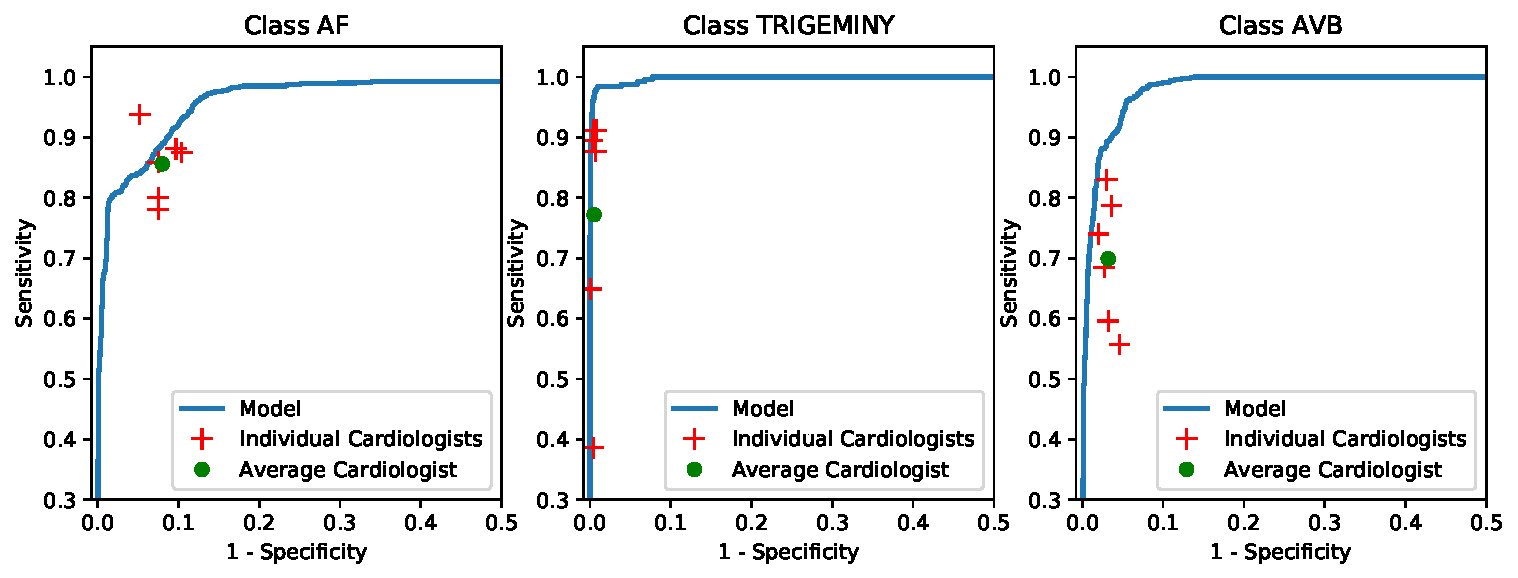
\includegraphics[width=1.0\textwidth]{arrhythmias/figures/roc_curve.pdf}
\caption{Receiver operating characteristic curves at sequence-level for atrial
         fibrillation (AF), trigeminy and atrioventricular block (AVB).}
\label{fig:arrhythmias:roc_curve}
\end{figure}

\begin{figure}
\centering
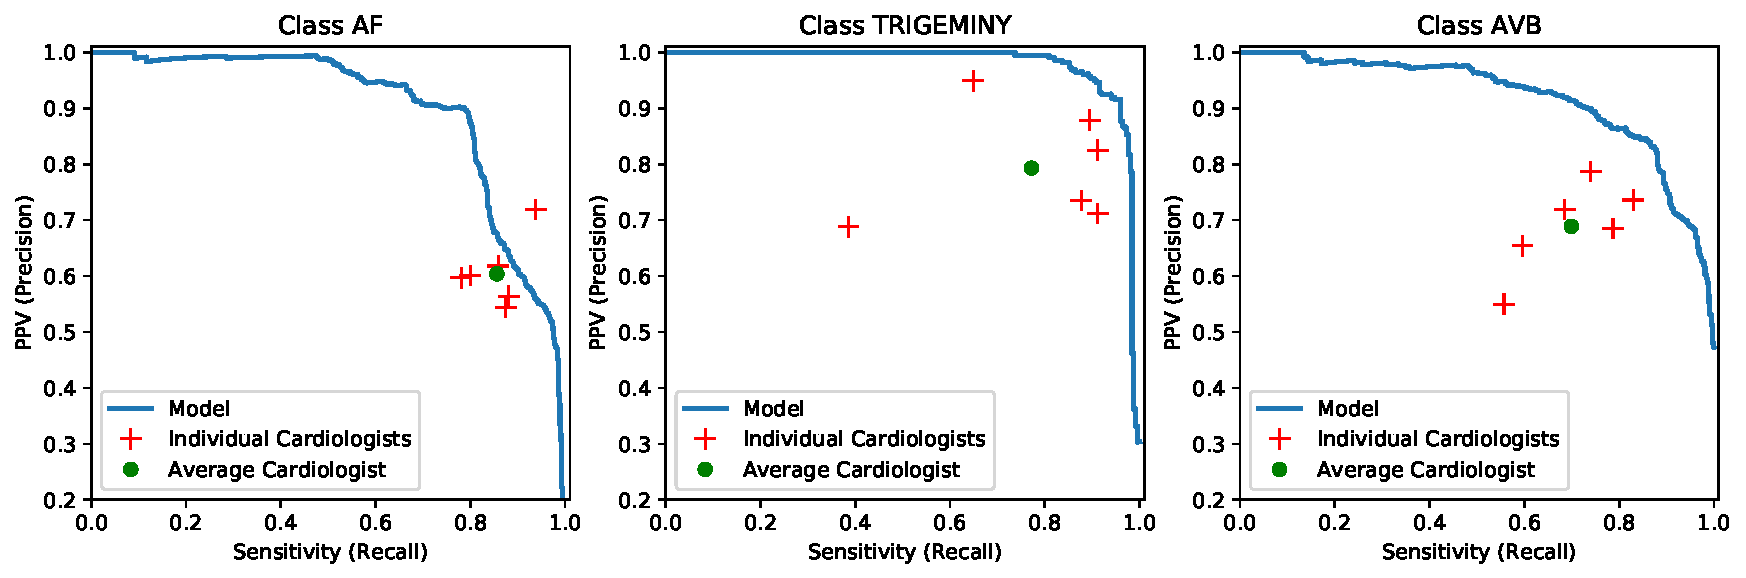
\includegraphics[width=1.0\textwidth]{arrhythmias/figures/prec_recall_curve.pdf}
\caption{Precision-Recall curves at sequence-level for atrial fibrillation,
         trigeminy and atrioventricular block.}
\label{fig:arrhythmias:prec_recall_curve}
\end{figure}
